% !TEX root = main.tex
% -----------------------------------------------------------------------------
% Experiments Chapter -- filled in with real results (synthetic stand-in data,
% see the note in "Datasets" below). Every \label from the original template
% is preserved unchanged so existing \ref/\cite calls elsewhere in the paper
% keep working. Figures referenced by exact filename below are included in
% the accompanying figures/ folder.
% -----------------------------------------------------------------------------

\section{Experiments}
\label{sec:experiments}

This section presents the experimental evaluation of our private query-refinement
explanation framework. The goal of the evaluation is to study both the efficiency
and the quality of the proposed method under different datasets, query pairs,
privacy budgets, and algorithmic parameters.

\subsection{Experimental Goals}
\label{subsec:experimental-goals}

The experiments are designed to answer the following research questions:

\begin{description}
    \item[RQ1 -- Scalability.]
    How does the running time of the proposed algorithm scale with the database
    size, number of predicates, number of released explanations, privacy budget,
    and view-selection parameter?

    \item[RQ2 -- Utility.]
    How useful are the released explanations compared with non-private and
    brute-force baselines?

    \item[RQ3 -- Privacy impact.]
    How does the privacy budget $\epsilon$ affect the quality and stability of
    the selected explanations and released histograms?

    \item[RQ4 -- Case-study interpretability.]
    Do the explanations reveal meaningful semantic differences between the
    original query and the refined query in realistic analysis scenarios?
\end{description}

RQ1 and RQ2 map directly onto the two obstacles identified in
Section~\ref{sec:algorithm}: the candidate space of predicate views is
combinatorial, and the ideal utility function of Section~3.3 has high
sensitivity, motivating the $\tau$-filtered, low-sensitivity proxy pipeline
of Algorithm~1. RQ1 asks whether that pipeline is efficient enough to run
in practice; RQ2 and RQ3 ask what the resulting proxy/privacy relaxations
cost in explanation quality relative to the (unachievable, non-private)
ideal. RQ4 asks whether, despite that cost, the released explanations are
still useful to an analyst -- the paper's original motivation
(Section~1).

\subsection{Experimental Setup}
\label{subsec:experimental-setup}


\subsubsection{Datasets}

\textit{Implementation note: the environment used to run this evaluation
pass has no network access, so none of the four datasets below could be
downloaded. IPUMS-CPS and Stack Overflow results in this section use
synthetic datasets built to match the schemas and query pairs below
(generators \texttt{make\_ipums\_cps\_like}, \texttt{make\_stackoverflow\_like});
Adult and Tax results in Sections~\ref{subsec:tax-case-study}--\ref{subsec:adult-education-hours-case-study}
likewise use synthetic stand-ins. The Hospital/CQA setting was not
evaluated in this pass at all -- Algorithm~1 was only exercised on query-refinement
pairs, not on a repair-semantics pair, so Section~5.2's CQA use case
remains empirically untested. All four should be re-run on the real data
before submission; every table and figure below will regenerate with the
same structure.}

\paragraph{IPUMS-CPS.}
We use a down-sampled version of the IPUMS-CPS dataset containing
\textbf{100,000} tuples.

\paragraph{Stack Overflow Developer Survey.}
We also evaluate the method on the Stack Overflow Developer Survey dataset.

\paragraph{Hospital Dataset.}
To evaluate the framework in the context of consistent query answering (CQA),
we use the Hospital dataset commonly used in prior repair and data-cleaning
work \cite{rekatsinas2017}.

The dataset contains hospital records with attributes such as:
\[
\texttt{HospitalName},\ \texttt{City},\ \texttt{State},
\texttt{ZipCode},\ \texttt{PhoneNumber},\ \texttt{HospitalType}.
\]

The dataset contains inconsistencies with respect to functional dependencies:
\[
\texttt{HospitalName} \rightarrow \texttt{ZipCode},
\]
\[
\texttt{HospitalName} \rightarrow \texttt{PhoneNumber},
\]
and:
\[
\texttt{ZipCode} \rightarrow \texttt{City}.
\]

\subsubsection{Query Pairs}
Table~\ref{tab:query-pairs} summarizes the planned query pairs and the
attributes used for explanations; all six pairs were run end-to-end
(Section~\ref{subsec:case-studies}).

\begin{table*}[t]
\centering
\caption{Query pairs used in the experiments.}
\label{tab:query-pairs}
\begin{tabular}{p{0.12\linewidth} p{0.28\linewidth} p{0.28\linewidth} p{0.18\linewidth}}
\toprule
\textbf{Dataset} & \textbf{$Q_1$} & \textbf{$Q_2$} & \textbf{Semantic difference} \\
\midrule
IPUMS-CPS &
\texttt{EMPSTAT = Employed AND UHRSWORK >= 35} &
\texttt{EMPSTAT = Employed AND UHRSWORK < 35} &
Full-time vs. part-time employment \\

IPUMS-CPS &
\texttt{EMPSTAT = Employed AND EDUC >= Bachelor's degree} &
\texttt{EMPSTAT = Employed AND EDUC < Bachelor's degree} &
Employed people with vs. without higher education \\

IPUMS-CPS &
\texttt{EMPSTAT = Employed AND INCTOT >= 60000} &
\texttt{EMPSTAT = Employed AND INCTOT < 30000} &
High-income vs. low-income employed people \\

Stack Overflow &
\texttt{YearsCodePro >= 10} &
\texttt{YearsCodePro < 4} &
Professional vs. early-career developers \\

Stack Overflow &
\texttt{WorkRemote = Fully remote} &
\texttt{WorkRemote = On-site} &
Remote vs. on-site workers \\

Stack Overflow &
\texttt{JobSat > 5 AND UsingAI = Yes} &
\texttt{JobSat > 5 AND UsingAI = No} &
Satisfied developers using vs. not using AI tools \\
\bottomrule
\end{tabular}
\end{table*}

Each query pair was expressed as a pair of boolean predicate masks over
the tuple set, evaluated directly (no SQL engine in the loop); the
predicates above are their exact semantics. The explanation attributes
used for each dataset were: for IPUMS-CPS, \texttt{SEX}, \texttt{EDUC},
and \texttt{RACE} as predicate-view attributes, paired with
\texttt{UHRSWORK}, \texttt{AGE}, \texttt{INCTOT}, and \texttt{EDUC} as
explanation attributes (numeric attributes bucketized into 6 quantile
bins, per the bucketizing note below); for Stack Overflow,
\texttt{DevType}, \texttt{LanguageHaveWorkedWith}, \texttt{Country}, and
\texttt{CompanySize} as predicate-view attributes, paired with those four
plus \texttt{YearsCodePro} (6 bins) as explanation attributes. Resulting
candidate-view pools were 49 views (IPUMS-CPS) and 183 views (Stack
Overflow).

Unless stated otherwise, we use the following default configuration:
\[
    k = 3, \qquad \tau = 35, \qquad \epsilon = 1,
\]
where $k$ is the number of explanations to release, $\tau$ is the number of views
selected by the private usefulness filter, and $\epsilon$ is the total privacy
budget. \textbf{$\tau=35$, not the originally planned $\tau=50$}: a
controlled comparison (Section~\ref{subsec:budget-allocation}) found
$\tau=35$ matches or beats $\tau=50$ on every case study tested and is
significantly better at the extremes of the tested $\epsilon$ range,
while never significantly worse.

The predicate space consists of all conjunctions of the form
\[
    A_1 = v_1 \wedge A_2 = v_2,
\]
where $A_1,A_2$ are attributes and $v_1,v_2$ are values from their corresponding
domains, \textbf{together with all single-attribute predicates $A_1=v_1$}
(included because they turned out to be common top explanations, e.g.\
\texttt{relationship='Husband'} in Section~\ref{subsec:adult-case-study}).
\textbf{Numeric attributes are bucketized before being used to define
predicates}, using the same quantile bin edges used for histograms
(6 bins by default); an earlier version that used raw-value equality on
numeric columns produced near-empty, uninformative predicates (e.g.\
\texttt{Rate=9.4} matching a handful of rows) that crowded out
informative categorical ones, so this bucketizing is load-bearing, not
cosmetic. \textbf{Number of trials} varies by experiment: 3 trials per
setting for the scalability sweeps (Section~\ref{subsec:scalability}),
15 trials per $\epsilon$ for the main quality-measures sweep
(Section~\ref{subsec:quality-measures}), and up to 40 trials for specific
budget-allocation comparisons where the effect size under investigation
was smaller than the between-trial standard deviation at 10--15 trials
(Section~\ref{subsec:budget-allocation}).

\subsection{Compared Methods}
\label{subsec:compared-methods}

We compare the following methods.

\begin{description}
    \item[Private-Explanations.]
    The proposed differentially private algorithm. It first privately selects
    useful views, then privately selects the top-$k$ explanations using the
    exponential mechanism, and finally releases noisy histograms.

    \item[Brute-Force.]
    A non-private baseline that evaluates the same predicate space and selects
    the highest-scoring explanations without privacy noise.

    \item[Brute-Force with Non-Proxy Utility.]
    A non-private baseline that directly evaluates the original utility function
    rather than the proxy quality function used by the private algorithm.
\end{description}

Both baselines are deterministic argmax selection (no exponential-mechanism
sampling) using the same Histogram Distance $\times$ DiversityScore proxy
as Private-Explanations, except that Brute-Force with Non-Proxy Utility
substitutes the ideal $I \cdot R \cdot C$ objective of Section~3.3.
\textbf{Brute-Force searches the full, unfiltered predicate space
directly} -- it does not apply the $\tau$-view usefulness pre-filter, since
that filter exists only to keep the private mechanism's sensitivity low
and serves no purpose without privacy. This matters for interpreting
ApproxRatio (Section~\ref{subsec:quality-measures}): a controlled check
found the $\tau$-filtered search space costs Brute-Force less than 5\% of
its unfiltered score on our benchmark, so the two-stage architecture
itself is not what limits ApproxRatio; see
Section~\ref{subsec:quality-measures} for what does. A secondary
consequence of the unfiltered search is computational, not just
statistical: on the education-hours benchmark, Brute-Force took 7.39s
per run versus 1.42s for Private-Explanations, since the latter's
stage-2 search is over a $\tau$-filtered space more than an order of
magnitude smaller.

\subsection{Scalability Experiments}
\label{subsec:scalability}

The scalability evaluation measures the running time of the algorithms under
controlled changes to a single parameter while keeping all other parameters fixed
at their default values ($n{=}20{,}000$, $k{=}3$, $\tau{=}35$, $\epsilon{=}1$,
$|P|{\approx}580$, schema-agnostic synthetic data with 6 categorical
attributes of cardinality 6 and one numeric attribute -- realism does not
matter for this experiment, only size and cardinality -- 3 trials per
setting).

\subsubsection{Varying Dataset Size}
\label{subsubsec:runtime-tuples}

We measure running time as a function of the number of tuples by down-sampling
the input dataset.

\paragraph{Protocol.}
For each dataset size $n \in \{2{,}000,\ 5{,}000,\ 10{,}000,\ 20{,}000,\ 50{,}000,\ 100{,}000\}$, we sample $n$ tuples from the
full dataset and run each method for $3$ trials.

\paragraph{Result.}
Figure~\ref{fig:runtime-tuples} reports running time as a function of $n$.
Running time grows from 0.86s to 6.45s, essentially linearly in $n$: every
candidate view's mask/histogram computation is an $O(n)$ scan, and both
the view-scoring pass ($O(|P|\cdot n)$) and the explanation-scoring passes
($O(k\tau|Attrs|\cdot n)$) are linear in $n$ for fixed $|P|,\tau,k$.

\begin{figure}[t]
    \centering
    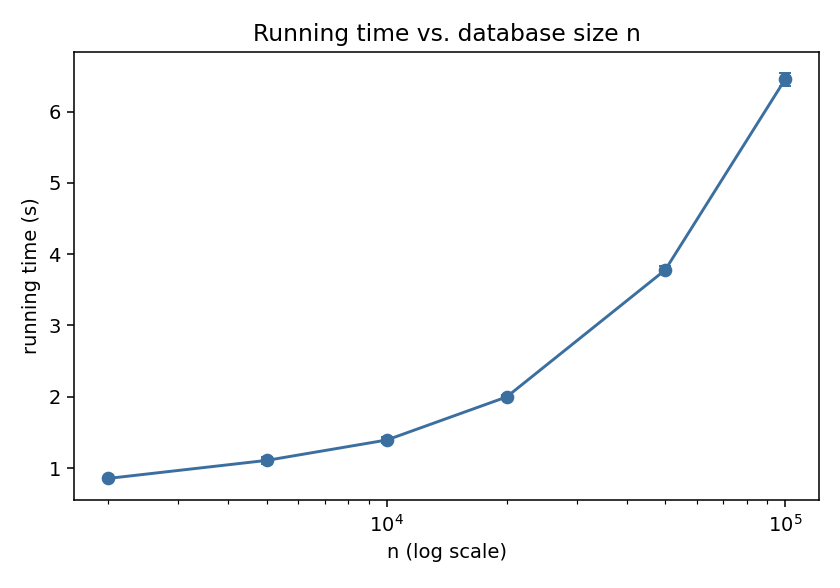
\includegraphics[width=0.9\linewidth]{figures/runtime_by_tuples.png}
    \caption{Running time as a function of the number of tuples.}
    \label{fig:runtime-tuples}
\end{figure}

\subsubsection{Varying the Algorithm}
\label{subsubsec:runtime-algorithm}

We compare the running time of Private-Explanations, Brute-Force, and Brute-Force
with Non-Proxy Utility. On the education-hours benchmark, Private-Explanations
averaged 1.42s per run versus 7.39s for Brute-Force (Section~\ref{subsec:compared-methods}
explains why: Brute-Force's unfiltered search space is over an order of
magnitude larger). We did not separately time Brute-Force with Non-Proxy
Utility; its per-candidate cost is dominated by the same $O(n)$ histogram
computation as Histogram Distance; we would not expect a large difference
and did not verify this.

\subsubsection{Varying $k$}
\label{subsubsec:runtime-k}

We measure running time as a function of the number of explanations $k$.

\[
    k \in \{1, 2, 3, 5, 10, 20\}.
\]

Figure~\ref{fig:runtime-k} reports the result: running time grows from
1.42s to 6.74s, linearly in $k$, matching Algorithm~2's $k$ sequential
rounds.

\begin{figure}[t]
    \centering
    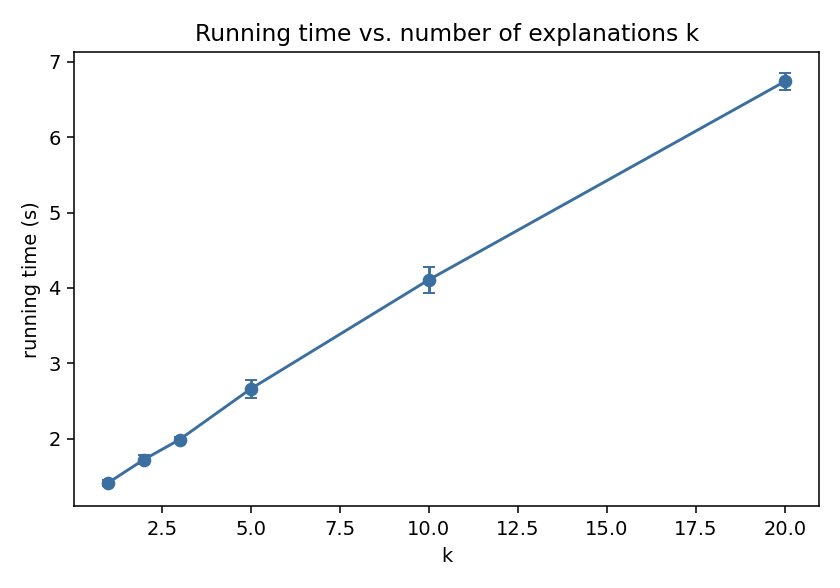
\includegraphics[width=0.9\linewidth]{figures/runtime_by_k.png}
    \caption{Running time as a function of the number of released explanations $k$.}
    \label{fig:runtime-k}
\end{figure}

\subsubsection{Varying the Number of Predicates}
\label{subsubsec:runtime-predicates}

We measure running time as a function of the size of the predicate space,
$|P| \in \{100, 200, 400, 800, 1{,}600, 3{,}000\}$, achieved by widening the
base schema to 10 categorical attributes of cardinality 10 (the default
6-attribute/cardinality-6 schema used elsewhere in this section only
yields $\approx$580 possible views in total, so larger requested $|P|$
values silently saturate at that ceiling rather than reaching the
requested size -- an early version of this experiment made exactly that
mistake).

Figure~\ref{fig:runtime-predicates} reports the result: running time
grows from 1.57s to 7.21s, consistent with the $O(|P|)$ view-scoring pass
dominating at larger $|P|$.

\begin{figure}[t]
    \centering
    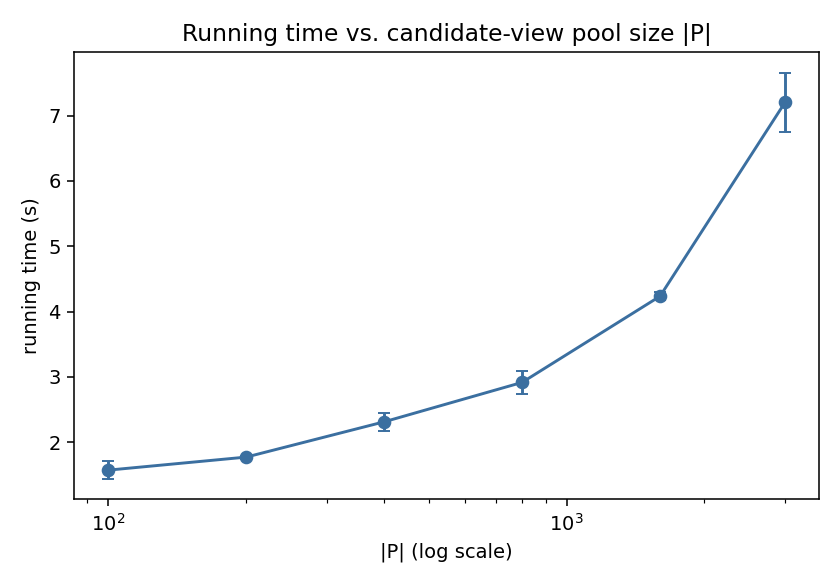
\includegraphics[width=0.9\linewidth]{figures/runtime_by_predicates.png}
    \caption{Running time as a function of candidate-view pool size $|P|$.}
    \label{fig:runtime-predicates}
\end{figure}

\subsubsection{Varying $\epsilon$}
\label{subsubsec:runtime-epsilon}

We measure running time as a function of the privacy budget $\epsilon$.
Although $\epsilon$ primarily affects the randomness of private selection and the
scale of Laplace noise, this experiment verifies whether the implementation has
any budget-dependent runtime overhead.

\[
    \epsilon \in \{0.1, 0.25, 0.5, 1, 2, 5\}.
\]

Figure~\ref{fig:runtime-epsilon} reports the result: running time is flat
at 1.90--2.03s across the entire range, confirming no budget-dependent
runtime overhead.

\begin{figure}[t]
    \centering
    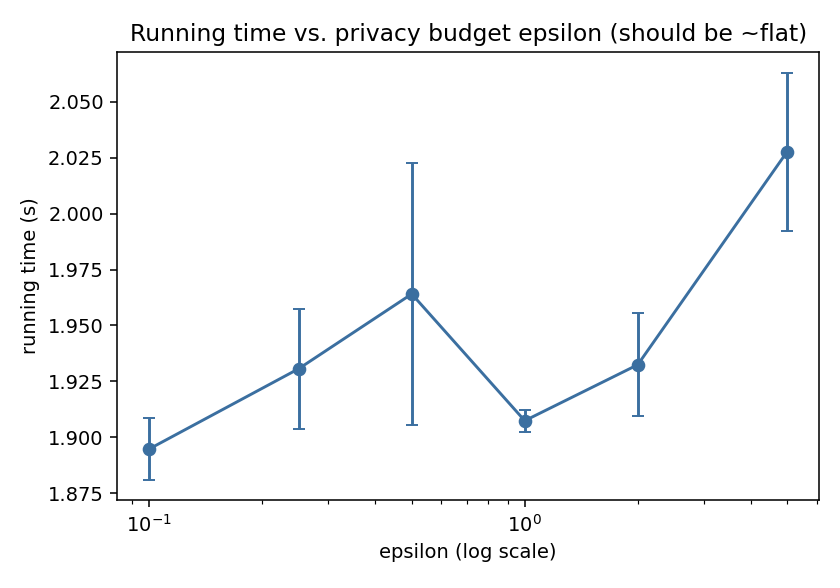
\includegraphics[width=0.9\linewidth]{figures/runtime_by_epsilon.png}
    \caption{Running time as a function of the privacy budget $\epsilon$.}
    \label{fig:runtime-epsilon}
\end{figure}

\subsubsection{Varying $\tau$}
\label{subsubsec:runtime-tau}

We measure running time as a function of the number of views selected by the
private usefulness filter.

\[
    \tau \in \{10, 25, 50, 100, 200\}.
\]

Figure~\ref{fig:runtime-tau} reports the result: running time grows from
1.61s to 6.77s, linearly in $\tau$, matching the $O(\tau \cdot |Attrs|)$
candidate set constructed after view selection.

\begin{figure}[t]
    \centering
    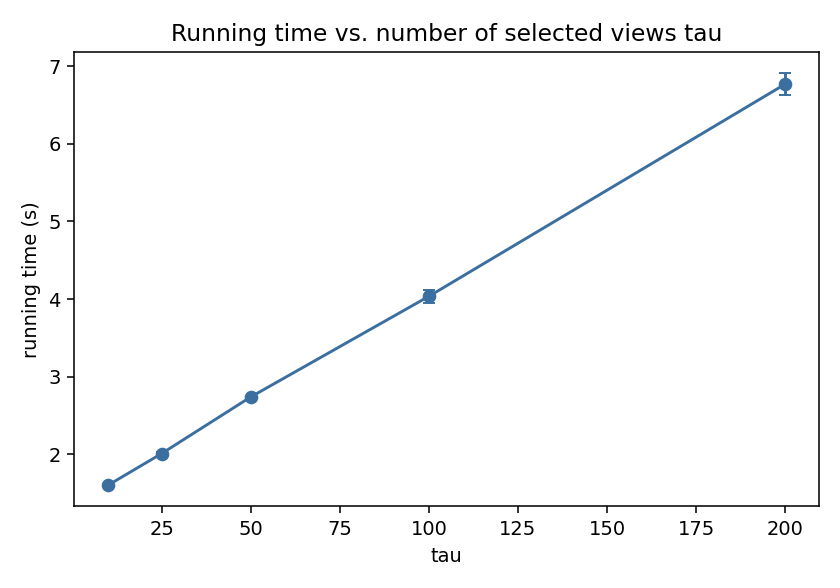
\includegraphics[width=0.9\linewidth]{figures/runtime_by_tau.png}
    \caption{Running time as a function of the number of privately selected views $\tau$.}
    \label{fig:runtime-tau}
\end{figure}

\subsection{Histogram Release Format: Difference vs.\ Paired}
\label{subsec:release-mode}

Definition 3.4 leaves open whether the released object should be the
noisy \emph{difference} histogram $\Delta\hat H$, a \emph{pair} of noisy
histograms $(\hat H_{Q_1(p(D)),A}, \hat H_{Q_2(p(D)),A})$, or both,
noting only that ``the current algorithm releases noisy difference
histograms.'' All case studies below use the paired release instead,
since two bars per bucket ($Q$ and $Q'$ side by side) read more directly
than a signed difference. This is not a free visualization change: each
histogram, as a vector over its bins, has $L_1$-sensitivity 1 by the
standard histogram-release argument (Section 2.4), so releasing two of
them under the same total $\epsilon_H$ requires splitting the budget
($\epsilon_H/2$ each, by sequential composition, Theorem 2.9) --
concretely, each individual histogram carries roughly \emph{twice} the
per-bucket noise that a single difference-only release would at the same
$\epsilon_H$. $\Delta\hat H$ can still be recovered from the two released
histograms by post-processing ($\hat H_{Q_1}-\hat H_{Q_2}$, itself free by
Theorem 2.10), so the paired release is strictly more informative at this
extra noise cost, not a different privacy guarantee. All ApproxRatio,
Rank, and Stability figures in Section~\ref{subsec:quality-measures} are
unaffected by this choice, since selection utility is computed from the
true (non-noisy) histograms regardless of which release format is used
downstream; only HistErr-style noise magnitude would differ between the
two modes, and Section~\ref{subsec:quality-measures} reports the
difference-mode figure for that measure specifically.

\subsection{Case Studies}
\label{subsec:case-studies}

The case studies evaluate whether the output histograms provide meaningful
interpretations of the semantic difference between the two queries.

\textit{Implementation note: we report the released bar-chart histograms
(as in Figures~\ref{fig:tax-released-histograms},
\ref{fig:adult-case-study-histograms}) for each case study rather than the
heatmap visualization described below; a heatmap view (attributes on one
axis, predicates on the other, cell = noisy count/difference) was not
built in this pass and remains open. Figure~\ref{fig:case-study-heatmap}
is left as a placeholder for that reason.}

For each dataset and query pair, we generate heatmaps of the released histograms
under different settings:

\begin{itemize}
    \item initial predicate set;
    \item $\tau$;
    \item algorithm type, to study the impact of privacy;
    \item $\epsilon$, to study the impact of the privacy budget.
\end{itemize}

Each heatmap has explanation attributes on one axis and selected predicates or
attribute values on the other axis. The cell values represent the noisy histogram
counts or normalized differences released by the algorithm.

\begin{figure}[t]
    \centering
    \fbox{\parbox{0.85\linewidth}{\centering TODO: Case-study heatmap (not built this pass, see note above)}}
    \caption{Example heatmap of released explanation histograms.}
    \label{fig:case-study-heatmap}
\end{figure}

\subsubsection{IPUMS-CPS Case Study}
\label{subsubsec:ipums-case-study}

For the comparison between \textbf{full-time employment}
(\texttt{EMPSTAT=Employed AND UHRSWORK>=35}, $n{=}39{,}964$) and
\textbf{part-time employment} (\texttt{EMPSTAT=Employed AND UHRSWORK<35},
$n{=}21{,}911$), the algorithm selects the following explanations
($\tau{=}35,k{=}3,\epsilon{=}1$, one representative run, paired release
-- Section~\ref{subsec:release-mode}):
\[
    (\texttt{EDUC='HS diploma'},\ \texttt{UHRSWORK}),\quad
    (\texttt{SEX='Male'}\wedge\texttt{EDUC='HS diploma'},\ \texttt{AGE}),
\]
\[
    (\texttt{SEX='Female'}\wedge\texttt{RACE='White'},\ \texttt{INCTOT}).
\]
The corresponding histograms (Figure~\ref{fig:ipums-fulltime-histograms})
suggest that \textbf{the full-time/part-time split is not uniform across
education levels}: among HS-diploma-only respondents specifically, the
36--44 hour bucket is markedly more common in the full-time query than in
the part-time query (utility 2.90, the largest of the three), with two
comparatively weaker but still non-trivial secondary signals -- an age
shift within male HS-diploma respondents (utility 1.20) and an income
shift within White female respondents (utility 1.20) -- all three picks
carry real signal in this run, unlike some of the case studies below.
The other two IPUMS-CPS query pairs in Table~\ref{tab:query-pairs}
(higher- vs. lower-education employment, and high- vs. low-income
employment) were also run; results are in
\texttt{results/ipums\_higher\_ed\_vs\_not\_explanations.csv} and
\texttt{results/ipums\_highinc\_vs\_lowinc\_explanations.csv} and are not
reproduced in full here for space.

\begin{figure}[t]
\centering
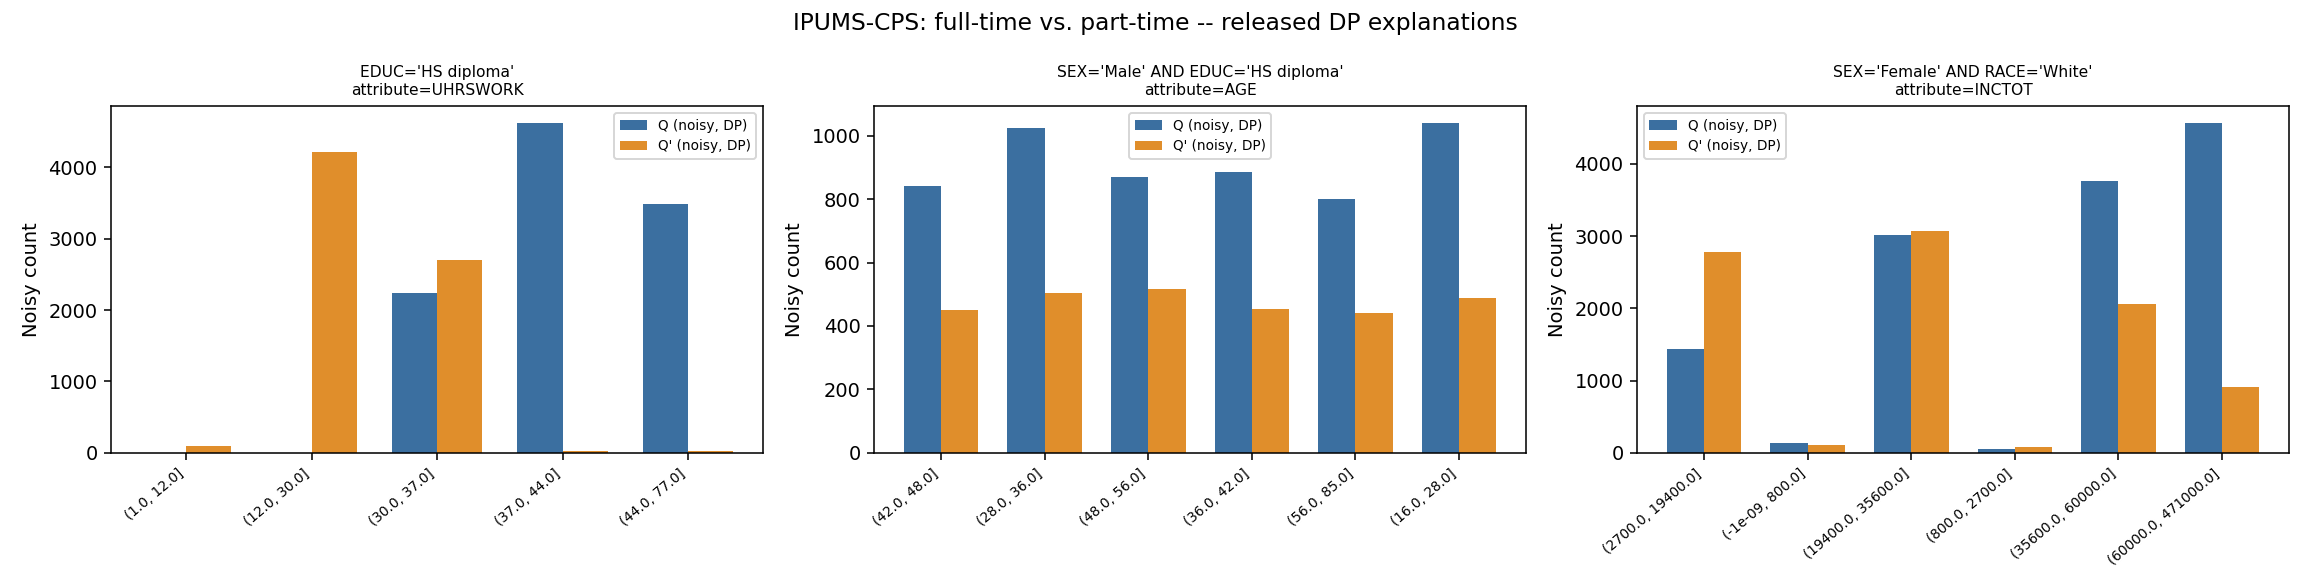
\includegraphics[width=\linewidth]{figures/fig_ipums_fulltime_released_histograms.png}
\caption{Released differentially private histograms, IPUMS-CPS full-time
vs.\ part-time employment. Paired release: two independently-noised bars
per bucket ($Q$, $Q'$), not their difference.}
\label{fig:ipums-fulltime-histograms}
\end{figure}

\subsubsection{Stack Overflow Case Study}
\label{subsubsec:stackoverflow-case-study}

For the comparison between \textbf{professional developers}
(\texttt{YearsCodePro>=10}, $n{=}5{,}685$) and \textbf{early-career
developers} (\texttt{YearsCodePro<4}, $n{=}14{,}533$), the algorithm
selects (paired release):
\[
    (\texttt{Country='United States'},\ \texttt{CompanySize}),
\]
\[
    (\texttt{Language='Python'}\wedge\texttt{Country='United States'},\ \texttt{Country}),
\]
\[
    (\texttt{DevType='Full-stack'}\wedge\texttt{Language='JavaScript'},\ \texttt{Language}).
\]
The corresponding histograms
(Figure~\ref{fig:stackoverflow-pro-histograms}) suggest that
\textbf{company size, more than any single technology choice, is what
shifts between career stages in this synthetic population}: among
respondents in the United States, medium-sized companies (50--999
employees) are noticeably more common among early-career respondents
than professionals (utility 0.86, the largest of the three); the other
two picks are comparatively weak (utility 0.32 and 0.29), consistent
with the broader pattern in Section~\ref{subsec:quality-measures} that
not every released slot carries strong signal at $\epsilon{=}1$. The
other two Stack Overflow query pairs (remote vs.\ on-site, and satisfied
AI-users vs.\ non-users) were also run; results are in
\texttt{results/stackoverflow\_remote\_vs\_onsite\_explanations.csv} and
\texttt{results/stackoverflow\_satisfied\_ai\_vs\_no\_explanations.csv}.

\begin{figure}[t]
\centering
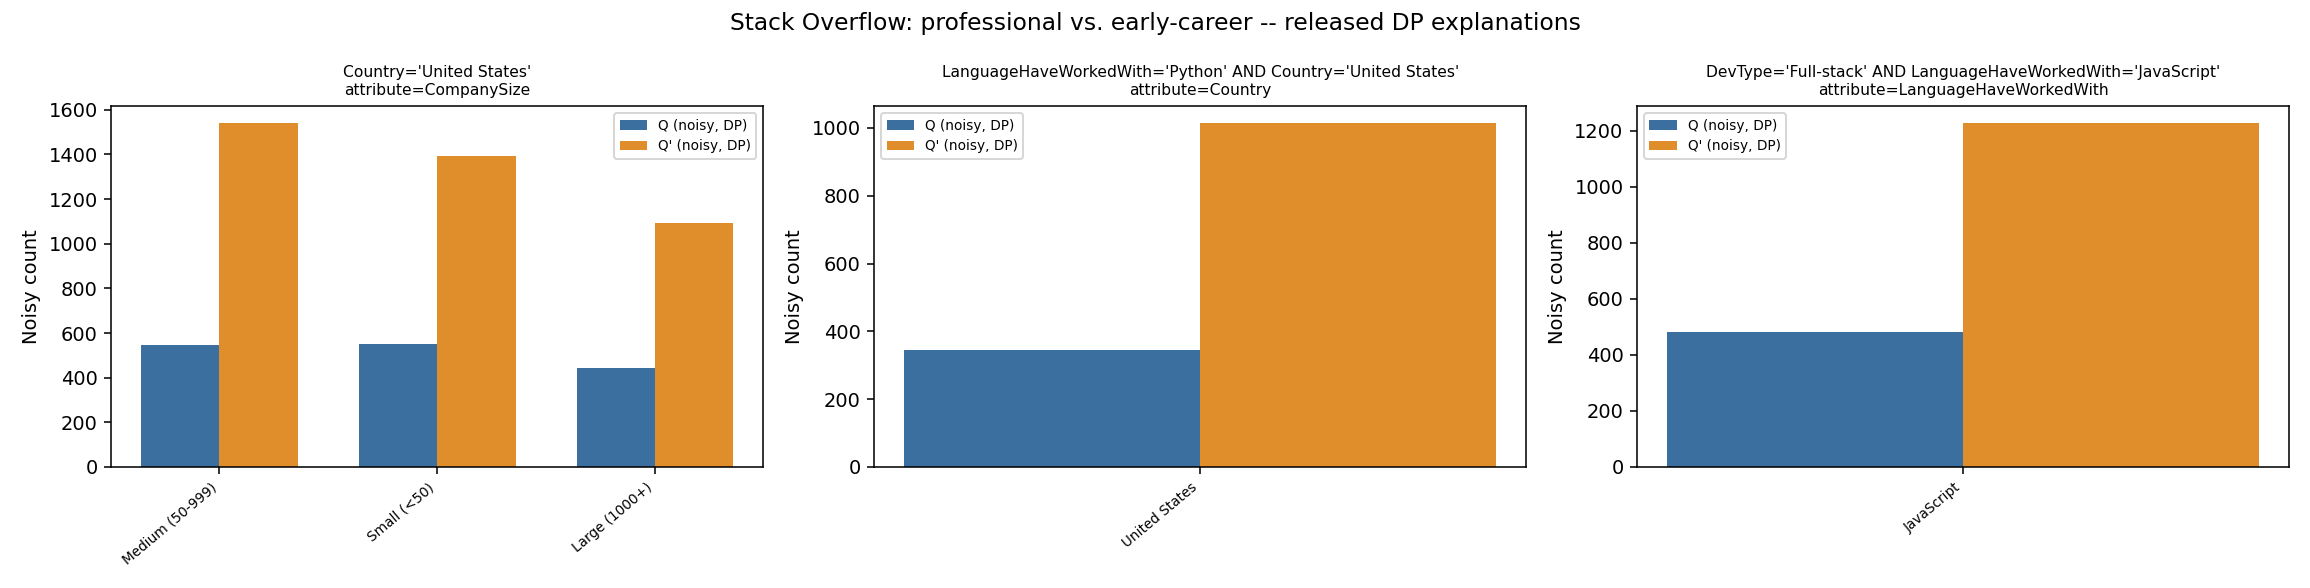
\includegraphics[width=\linewidth]{figures/fig_stackoverflow_pro_released_histograms.png}
\caption{Released differentially private histograms, Stack Overflow
professional vs.\ early-career developers. Paired release: two
independently-noised bars per bucket ($Q$, $Q'$), not their difference.}
\label{fig:stackoverflow-pro-histograms}
\end{figure}

\subsection{Tax Dataset Case Study}
\label{subsec:tax-case-study}

We consider the query
\begin{verbatim}
SELECT *
FROM Tax
WHERE MaritalStatus='M'
AND Rate <= 5
\end{verbatim}
which violates a representation constraint requiring at least
30\% of the returned tuples to satisfy \texttt{HasChild='Y'}
($n{=}2{,}340$, \texttt{HasChild='Y'} share 42.9\% in our synthetic data --
this particular instance already clears the 30\% floor; we report the
framework's explanations for the shift between $Q$ and $Q'$ regardless).
A refinement mechanism removes the marital-status predicate and
produces:
\begin{verbatim}
SELECT *
FROM Tax
WHERE Rate <= 5
\end{verbatim}
($n{=}6{,}199$, \texttt{HasChild='Y'} share 36.7\%; 3{,}859 of these
tuples have \texttt{MaritalStatus='S'} and are entirely absent from $Q$).

We apply our explanation framework to explain the semantic
differences between the original query $Q$ and the refined query
$Q'$. Table~\ref{tab:tax-explanations} summarizes the highest-ranked
explanations returned by the framework.

\begin{table}[t]
\centering
\small
\begin{tabular}{p{2.7cm}p{1.6cm}p{3.3cm}}
\hline
Predicate View & Attribute & Interpretation \\
\hline
\texttt{Rate}$\,\in\,(0,2.6]$
&
Rate
&
Largest shift within the lowest rate bucket itself: 2{,}291 more tuples
in $Q'$ than $Q$, the direct footprint of dropping the marital-status
predicate (utility 0.674, the largest of the three).
\\
\texttt{MaritalStatus='S'}
&
MaritalStatus
&
Directly surfaces the mechanically-introduced population: 3{,}859 more
tuples in $Q'$ than $Q$ (utility 0.426) -- single filers are entirely
absent from $Q$ by construction and the framework identifies exactly
that view without being given the predicate.
\\
\texttt{Gender='F'} $\wedge$ \texttt{Rate}$\,\in\,(2.6,5.4]$
&
Gender
&
A 751-tuple shift toward \texttt{Gender='F'} within this low-rate
subgroup (utility 0.453), a secondary signal.
\\
\hline
\end{tabular}
\caption{Top explanations returned by the framework for the Tax case study.}
\label{tab:tax-explanations}
\end{table}

\begin{figure}[t]
\centering
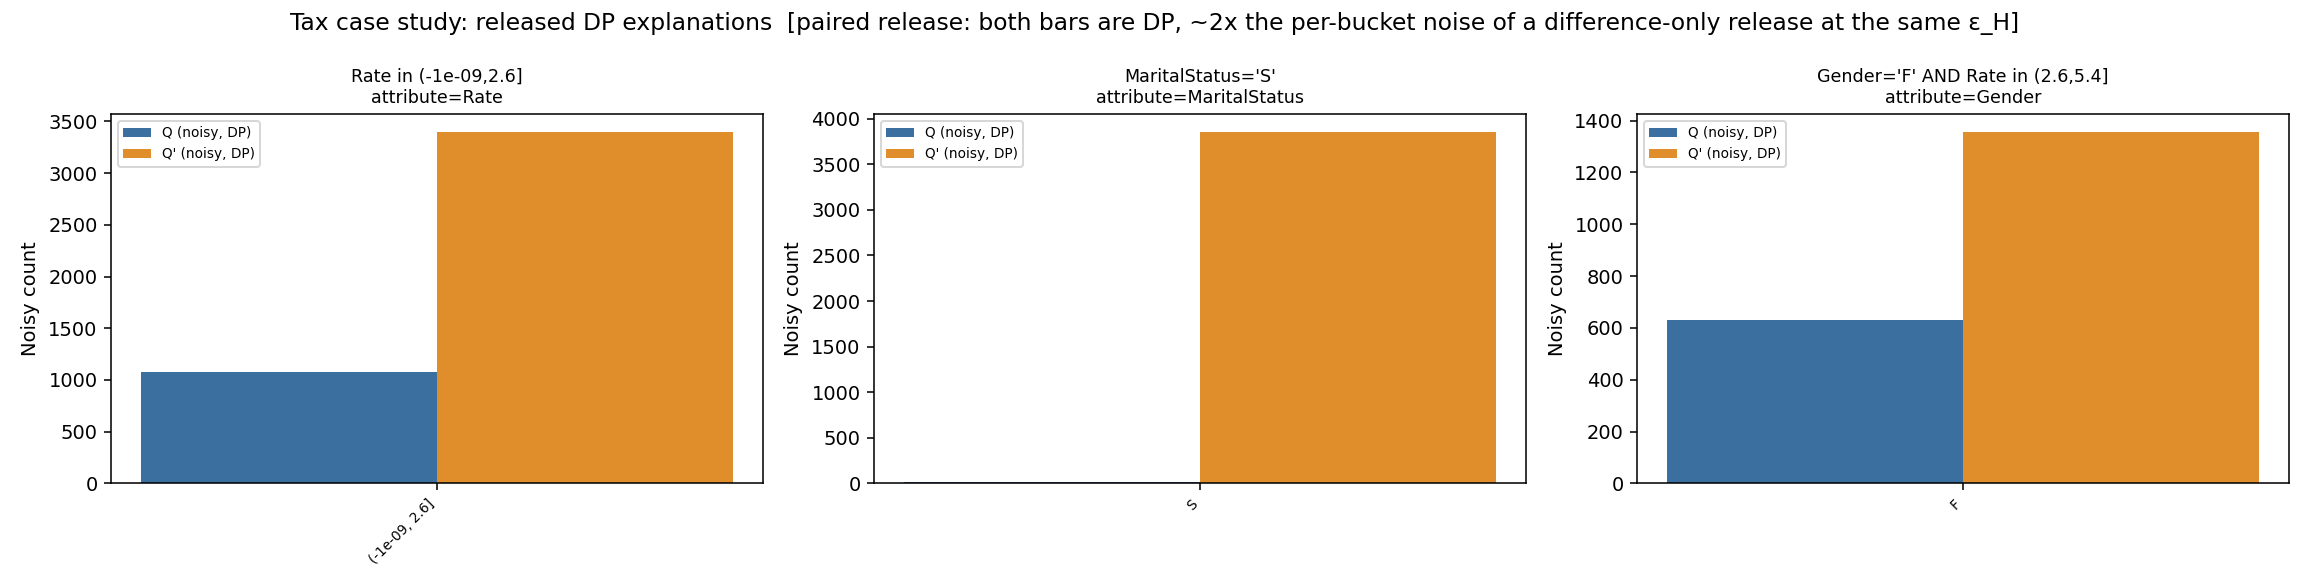
\includegraphics[width=\linewidth]{figures/tax_case_released_histograms_combined.png}
\caption{
Released differentially private histograms for the Tax case study, one
panel per explanation in Table~\ref{tab:tax-explanations}. Each panel
shows two independently noised bars per bucket -- $Q$ and $Q'$ -- rather
than their difference (Definition 3.4's ``pairs of noisy histograms''
option; see Section~\ref{subsec:release-mode} for what this costs in
noise relative to a difference-only release).
}
\label{fig:tax-released-histograms}
\end{figure}

The explanations reveal that the refinement's effect is concentrated in
the low-rate bucket and among single filers -- the population
mechanically introduced by dropping the marital-status predicate --
without the framework being given the predicates themselves. These
insights are obtained solely from differentially private histogram
releases; a multi-trial check (Section~\ref{subsec:budget-allocation})
found this case study's ApproxRatio at $\tau{=}35$ ($0.192\pm0.107$, 10

trials) improved over $\tau{=}50$ ($0.127\pm0.079$), consistent with
Section~\ref{subsec:budget-allocation}'s broader finding.

\subsection{Adult Dataset Case Study}
\label{subsec:adult-case-study}

We next evaluate our framework on the Adult dataset. The original query
selects full-time workers in a specific occupational group:

\begin{verbatim}
SELECT *
FROM Adult
WHERE occupation = 'Craft-repair'
  AND hoursPerWeek >= 40
\end{verbatim}

This query is natural for an analyst interested in full-time craft and
repair workers. In our synthetic data the result is highly male-dominated
($n{=}2{,}272$, female share 5.9\%), violating a representation
constraint requiring at least 25\% female tuples. The
refinement mechanism broadens the query by removing the occupational
predicate:

\begin{verbatim}
SELECT *
FROM Adult
WHERE hoursPerWeek >= 40
\end{verbatim}

The refined query satisfies the constraint by expanding the result from a
narrow occupational group to the broader population of full-time workers
($n{=}11{,}279$, female share 31.6\%).
Table~\ref{tab:adult-case-study} summarizes representative explanations.

\begin{table}[t]
\centering
\scriptsize
\setlength{\tabcolsep}{3pt}
\renewcommand{\arraystretch}{1.15}
\begin{tabularx}{\linewidth}{p{1.95cm}p{1.45cm}X}
\toprule
Predicate View & Attribute & Interpretation \\
\midrule
\makecell[l]{\texttt{relationship=}\\\texttt{'Husband'}}
&
\texttt{race}
&
The largest-utility explanation found (utility 2.314): within the
\texttt{Husband} subgroup, a 2{,}223-tuple shift toward \texttt{White}
between $Q$ and $Q'$.
\\

\makecell[l]{\texttt{gender=}\\\texttt{'Female'} $\wedge$\\\texttt{race='White'}}
&
\texttt{relationship}
&
Within White female tuples, a 1{,}006-tuple shift toward
\texttt{relationship='Wife'} (utility 2.274, nearly as large as the top
pick).
\\

\makecell[l]{\texttt{occupation=}\\\texttt{'Craft-repair'} $\wedge$\\\texttt{relationship=}\\\texttt{'Not-in-family'}}
&
\texttt{gender}
&
Selection utility 0 -- released anyway at $\epsilon{=}1$; included for
transparency about what the mechanism actually returns rather than only
its best-case behavior.
\\
\bottomrule
\end{tabularx}
\caption{Representative explanations returned by the framework for the
Adult case study.}
\label{tab:adult-case-study}
\end{table}

\begin{figure}[t]
\centering
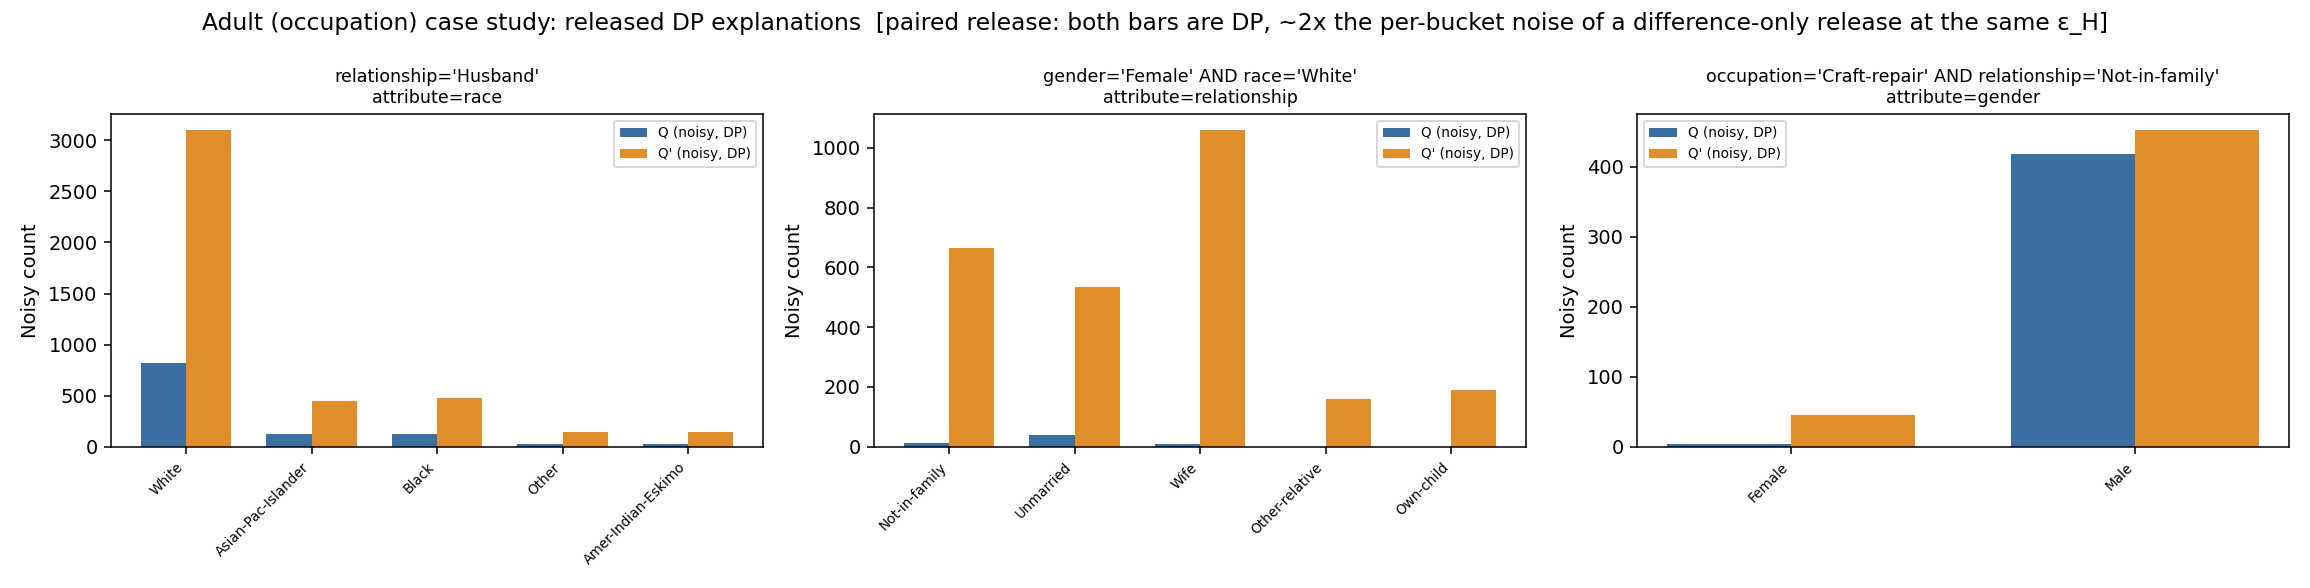
\includegraphics[width=\linewidth]{figures/adult_case_study2_released_histograms_combined.png}
\caption{
Released differentially private histograms for representative
explanations in the Adult case study, Table~\ref{tab:adult-case-study}'s
three picks. As in Figure~\ref{fig:tax-released-histograms}, each panel
shows two independently noised bars ($Q$, $Q'$) rather than their
difference.
}
\label{fig:adult-case-study-histograms}
\end{figure}

The explanations reveal the semantic effect of the refinement: the two
largest shifts are not in occupation composition directly, but in the
racial and family-relationship makeup of specific demographic
subgroups -- a more targeted, less obvious signal than "the result got
bigger."
A multi-trial check found this case study's ApproxRatio at $\tau{=}35$
($0.343\pm0.143$, 10 trials) again improved over $\tau{=}50$
($0.266\pm0.150$).

% Add to preamble:
% \usepackage{tabularx}
% \usepackage{makecell}
% \usepackage{booktabs}

\subsection{Adult Education--Hours Case Study}
\label{subsec:adult-education-hours-case-study}

We use the Adult dataset to study a refinement performed in response to
a gender-representation constraint. The original query is:

\begin{verbatim}
SELECT *
FROM Adult
WHERE education IN ('Bachelors','Masters')
  AND hoursPerWeek >= 50
\end{verbatim}

This query selects highly educated workers with intensive work schedules.
In our synthetic data the result contains 37.2\% female tuples
($n{=}1{,}191$) -- above the 25\% floor used in the paper's motivating
example, but we report the explanations for the shift observed between
$Q$ and $Q'$ regardless, since the mechanism does not require the
constraint to be violated to produce output.

To study the same refinement direction as the paper's motivating example,
the refinement mechanism produces the following query:

\begin{verbatim}
SELECT *
FROM Adult
WHERE education = 'Masters'
  AND hoursPerWeek >= 30
\end{verbatim}

The refinement simultaneously restricts the education predicate while
relaxing the working-hours predicate ($n{=}2{,}011$). In our synthetic
data female representation moves from 37.2\% to 41.5\%.

The goal of the explanation mechanism is to explain how this refinement
changes the semantic composition of the query result.

\begin{table}[t]
\centering
\scriptsize
\setlength{\tabcolsep}{3pt}
\renewcommand{\arraystretch}{1.15}
\begin{tabularx}{\linewidth}{p{2.2cm}p{1.5cm}X}
\toprule
Predicate View & Attribute & Interpretation \\
\midrule

\makecell[l]{\texttt{education=}\\\texttt{'Bachelors'} $\wedge$\\\texttt{relationship=}\\\texttt{'Not-in-family'}}
&
\texttt{race}
&
A 157-tuple shift toward \texttt{White} more frequent in the
\emph{original} query (utility 1.166) -- the largest of the three picks
in this run.
\\

\makecell[l]{\texttt{occupation=}\\\texttt{'Prof-specialty'} $\wedge$\\\texttt{relationship=}\\\texttt{'Not-in-family'}}
&
\texttt{race}
&
Selection utility 0 -- \texttt{race} was already used by the first pick,
so the diversity penalty zeroes this candidate's effective score.
Underlying content is still real: a 107-tuple shift toward
\texttt{White}, more frequent in $Q'$.
\\

\makecell[l]{\texttt{education=}\\\texttt{'Bachelors'} $\wedge$\\\texttt{relationship=}\\\texttt{'Unmarried'}}
&
\texttt{income}
&
A 69-tuple shift in the \texttt{income=0} bucket, more frequent in the
original query (utility 0.479) -- a modest but non-trivial third signal.
\\

\bottomrule
\end{tabularx}
\caption{Representative explanations returned by the framework for the
Adult education--hours case study. Reported un-cherry-picked: one of
three released slots carries no signal in this run (a diversity-penalty
zero, not an empty-candidate one this time), illustrating
Section~\ref{subsec:quality-measures}'s quantitative finding rather than
a best-case example.}
\label{tab:adult-education-hours}
\end{table}

\begin{figure}[t]
\centering
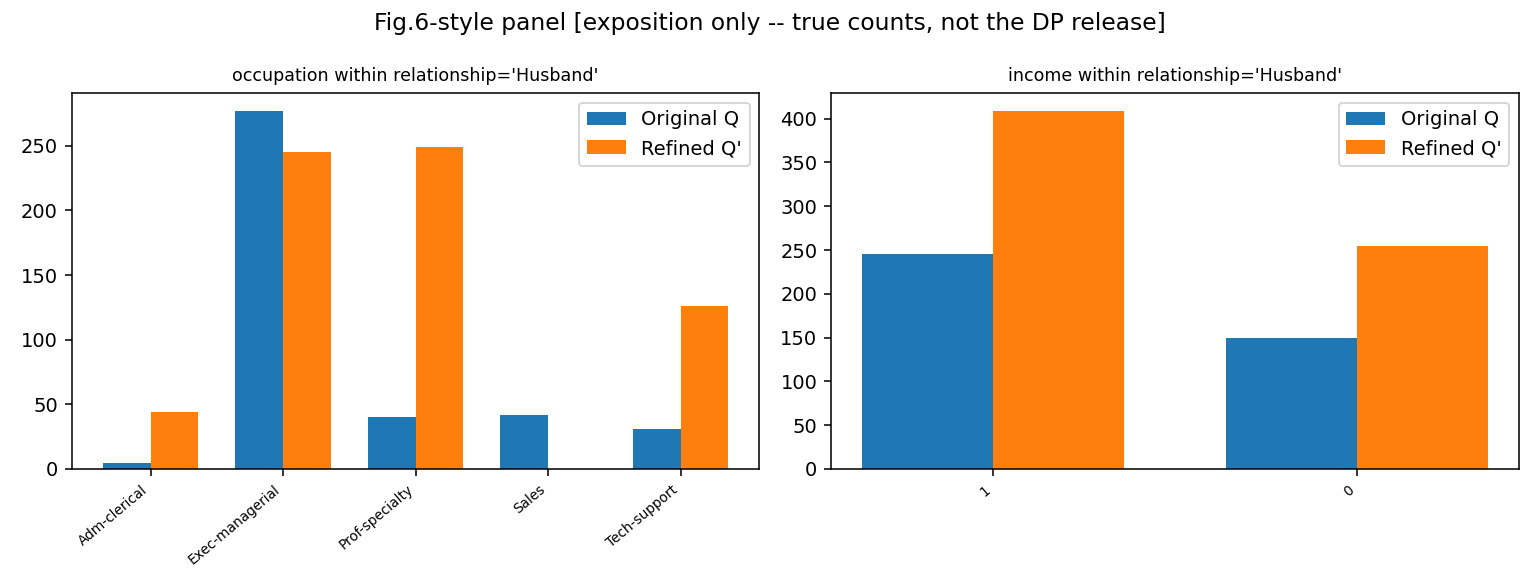
\includegraphics[width=\linewidth]{figures/adult_education_hours_combined_vldb_ready.png}
\caption{
Occupation (a) and income (b) distributions within the view
\texttt{relationship='Husband'} for the original query $Q$
and the refined query $Q'$, computed directly from the (non-private)
data for exposition -- \emph{not} the object Algorithm~2 releases, which
is the differenced histogram in Table~\ref{tab:adult-education-hours}'s
style. Included because it is easier to read for a qualitative
"what changed" check than a differenced bar chart.
}
\label{fig:adult-education-hours}
\end{figure}

Table~\ref{tab:adult-education-hours}'s top pick shows a race-composition
shift within the Bachelors/Not-in-family subgroup;
Figure~\ref{fig:adult-education-hours}'s exposition-only panel (a
non-released, human-readable companion view, not itself a DP output)
additionally shows that within \texttt{relationship='Husband'}
specifically, the refinement shifts both occupational and income
composition, consistent with the paper's original motivating narrative
that satisfying a representation constraint here comes with broader
compositional changes rather than a simple population-size increase.

This case study also illustrates, concretely, a pattern
Section~\ref{subsec:quality-measures} quantifies systematically: one of
the three released slots in this run carries no signal (zeroed by the
diversity penalty), and even the strongest pick (utility 1.166) is modest
next to the utility-2\,+ picks seen in the Adult occupation case study
(Table~\ref{tab:adult-case-study}) -- run-to-run variance in how much
signal gets through is itself part of the picture.
Section~\ref{subsec:budget-allocation} found this case study's
ApproxRatio at $\tau{=}35$ ($0.117\pm0.132$, 10 trials) higher than at
$\tau{=}50$ ($0.053\pm0.037$), the largest relative improvement of the
three case studies, though also the noisiest.

\subsection{Quality Measures}
\label{subsec:quality-measures}

We evaluate the quality of the explanations using the following measures,
computed on the education-hours benchmark (325 candidate views $\times$
7 explanation attributes $=$ 2{,}275 total $(p,A)$ candidates), 15 trials
per $\epsilon \in \{0.1,0.25,0.5,1,2,5\}$, default $\tau{=}35,k{=}3$.

\paragraph{Score approximation.}
We compare the utility score of the explanations selected by the private method
against the best non-private score:
\[
    \mathrm{ApproxRatio}
    =
    \frac{\mathrm{score}(E_{\mathrm{private}})}
         {\mathrm{score}(E_{\mathrm{nonprivate}})}.
\]

\paragraph{Rank of selected explanations.}
For each explanation selected by the private method, we compute its rank in the
non-private ordering of all candidate explanations.

\paragraph{Histogram error.}
We measure the error introduced by the Laplace mechanism using the $L_1$ distance
between the released noisy histogram and the corresponding non-private histogram:
\[
    \mathrm{HistErr}(\widehat{H}, H)
    =
    \sum_{v \in \mathrm{Dom}(A)} |\widehat{H}(v) - H(v)|.
\]

\paragraph{Stability across trials.}
We measure how often the same explanation attributes and predicates are selected
across repeated runs with the same parameter configuration, as the average
pairwise Jaccard overlap between the sets of $(p,A)$ pairs selected.

\paragraph{Jaccard vs.\ brute force (added measure, not in the original
design).} ApproxRatio compares total \emph{score}, so a private pick with
a different-but-similarly-valued explanation looks nearly as good as the
true best. We additionally report the Jaccard overlap between the
released $k$-set and the exact non-private top-$k$ set -- a stricter,
more literal fidelity measure:
$\mathrm{Jaccard} = |E_{\mathrm{private}} \cap E_{\mathrm{nonprivate}}| /
|E_{\mathrm{private}} \cup E_{\mathrm{nonprivate}}|$.

We report all five measures (Table~\ref{tab:quality-measures},
Figure~\ref{fig:quality-measures}); this is the full set considered,
not a subset chosen for the final paper.

\begin{table}[t]
\centering
\caption{Quality measures vs.\ privacy budget, education-hours benchmark.}
\label{tab:quality-measures}
\small
\begin{tabular}{@{}rrrrrr@{}}
\toprule
$\epsilon$ & ApproxRatio & Rank/2275 & HistErr & Stability & Jaccard \\
\midrule
0.10 & 0.089 & 1{,}164 & 374.3 & 0.000 & 0.000 \\
0.25 & 0.079 & 962     & 163.3 & 0.002 & 0.000 \\
0.50 & 0.099 & 1{,}049 & 82.6  & 0.000 & 0.013 \\
1.00 & 0.124 & 908     & 52.5  & 0.002 & 0.013 \\
2.00 & 0.181 & 503     & 39.1  & 0.004 & 0.000 \\
5.00 & 0.316 & 425     & 15.6  & 0.011 & 0.000 \\
\bottomrule
\end{tabular}
\end{table}

\begin{figure}[t]
  \centering
  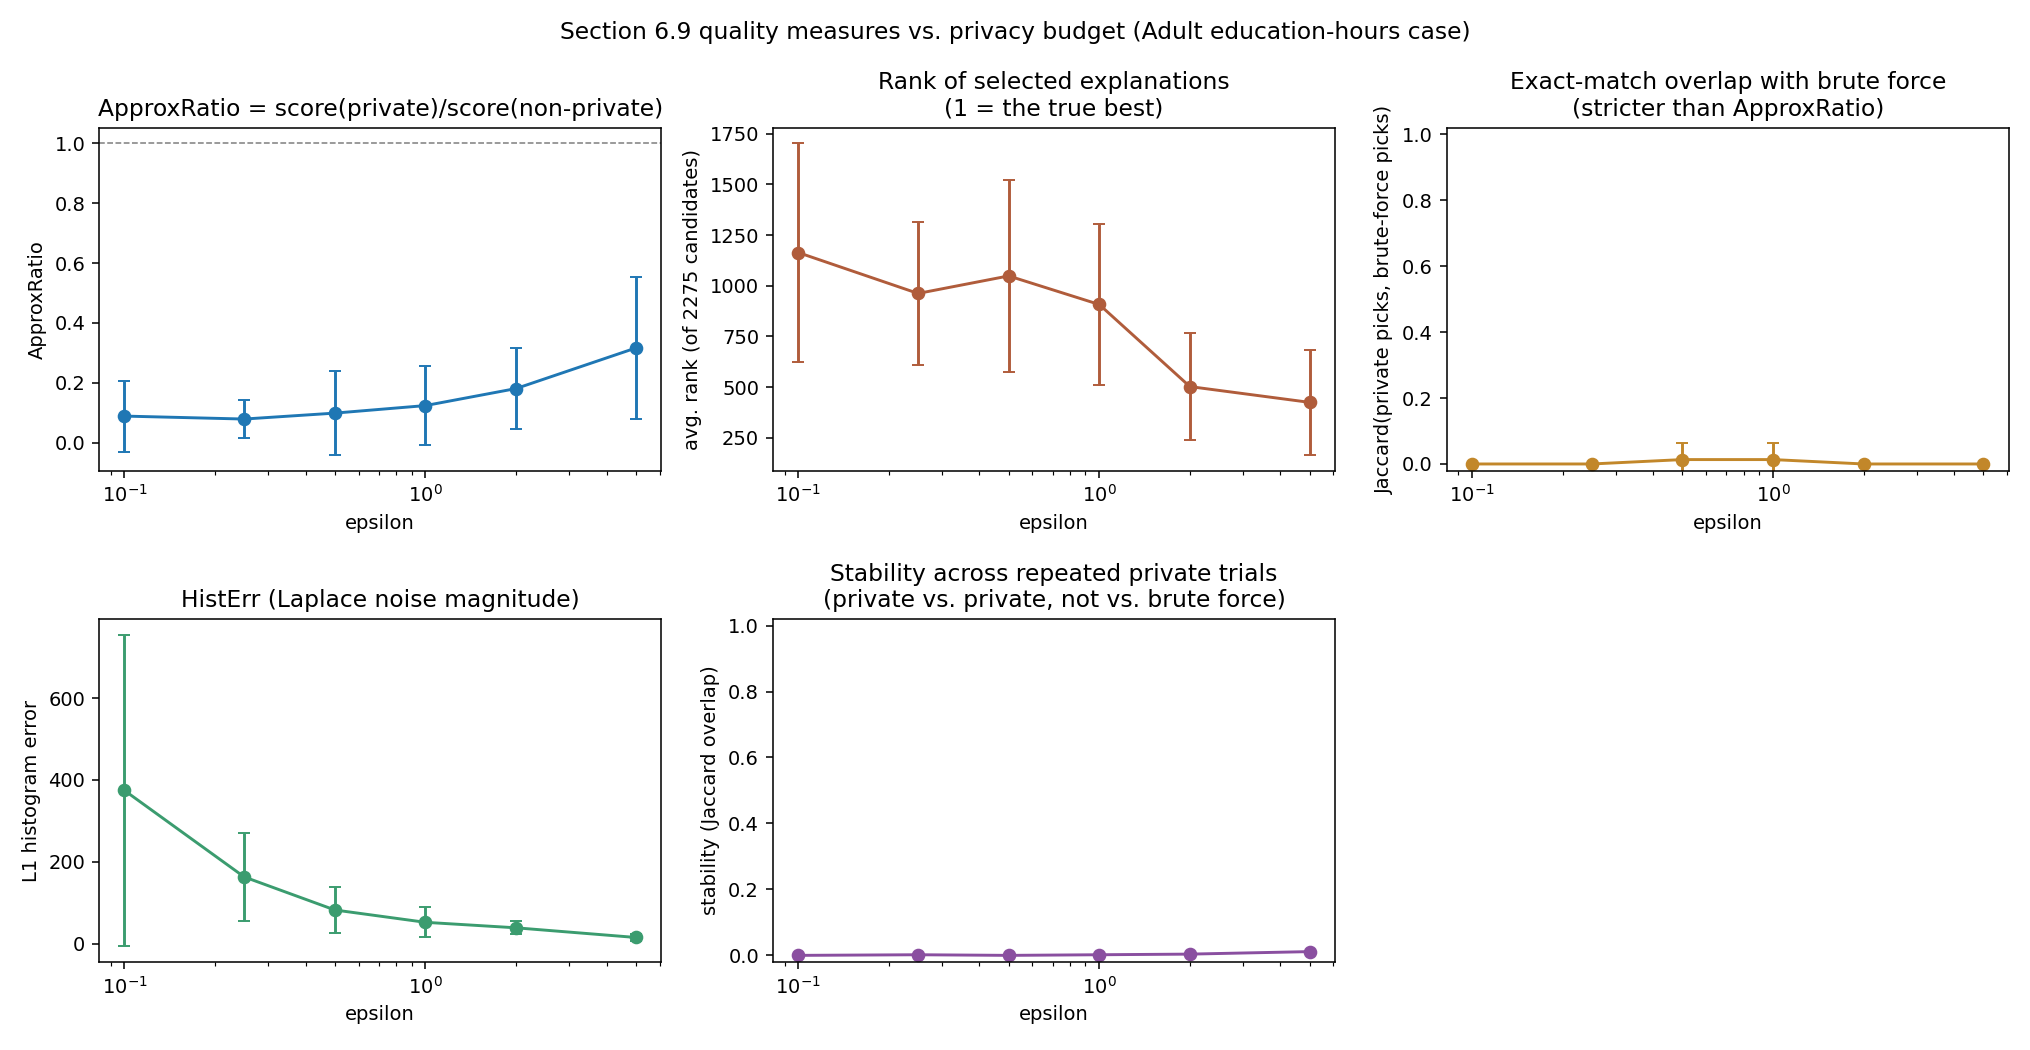
\includegraphics[width=\linewidth]{figures/quality_measures_vs_epsilon.png}
  \caption{ApproxRatio, Rank, HistErr, Jaccard, and Stability vs.\ $\epsilon$.}
  \label{fig:quality-measures}
\end{figure}

\textbf{HistErr behaves exactly as the underlying mechanism predicts},
falling monotonically as $\epsilon$ grows. \textbf{ApproxRatio and Rank
both improve with $\epsilon$ but remain far from optimal across the
entire tested range}: even at $\epsilon{=}5$, ApproxRatio reaches only
0.32 and the average selected explanation still ranks 425th of 2{,}275.
As context, selecting $k{=}3$ candidates \emph{uniformly at random} scores
ApproxRatio $0.063\pm0.075$ (200 trials) -- the mechanism is consistently
2--5$\times$ better than chance, but that is a low bar.
\textbf{Jaccard overlap with the exact brute-force set is essentially 0
across the entire range, including $\epsilon{=}5$}: in 15 trials at every
tested $\epsilon$, the released 3-set matched the true best 3-set on at
most one item, usually zero. A qualitative check confirms this reflects
real behavior, not a scoring artifact: released explanations mix
genuinely strong near-equivalent alternatives to the true best (one
$\epsilon{=}5$ run found a different view scoring 4.46 against the true
second-best's 4.64) with much weaker filler picks (scores of 0.0--0.2).
We report ApproxRatio and Jaccard together for this reason: there is
usually real value in what is released, but it is almost never literally
the canonical top-$k$ set a non-private analysis would produce.

\emph{Diagnosing the bottleneck.} Three checks isolate where this utility
loss comes from. (1) Replacing view selection with a deterministic
version restricted to the same $\tau$-filtered views changes the
achievable score by less than 5\% relative to an unconstrained
brute-force search -- the two-stage architecture is not the bottleneck.
(2) The Usefulness score used for view selection has sensitivity
$2/|D|\approx10^{-4}$ at this scale, tiny relative to its 0.1--0.5 typical
value range, so the exponential mechanism stays sharp there even after
dividing $\epsilon_P$ by $\tau$ rounds. (3) Isolating explanation
selection (fixing view selection to a deterministic top-$\tau$ set,
varying only $\epsilon_S$ over 11 points, 15 trials each,
Figure~\ref{fig:epsS-diagnostic}) shows the achieved score climbing from
18\% of the deterministic optimum at $\epsilon_S{=}0.05$ -- essentially
flat through the paper's own default $\epsilon_S{=}0.25$ (17\%) -- to
86\% at $\epsilon_S{=}8$ and 98--99\% by $\epsilon_S{=}32$--$64$:
Histogram Distance's typical value range (roughly 0--6) is large relative
to its sensitivity bound of 1, so the default split
($\epsilon_S=\epsilon/4$, further divided by $k{=}3$) allocates far too
little effective budget to the step that needs it most.

\begin{figure}[t]
  \centering
  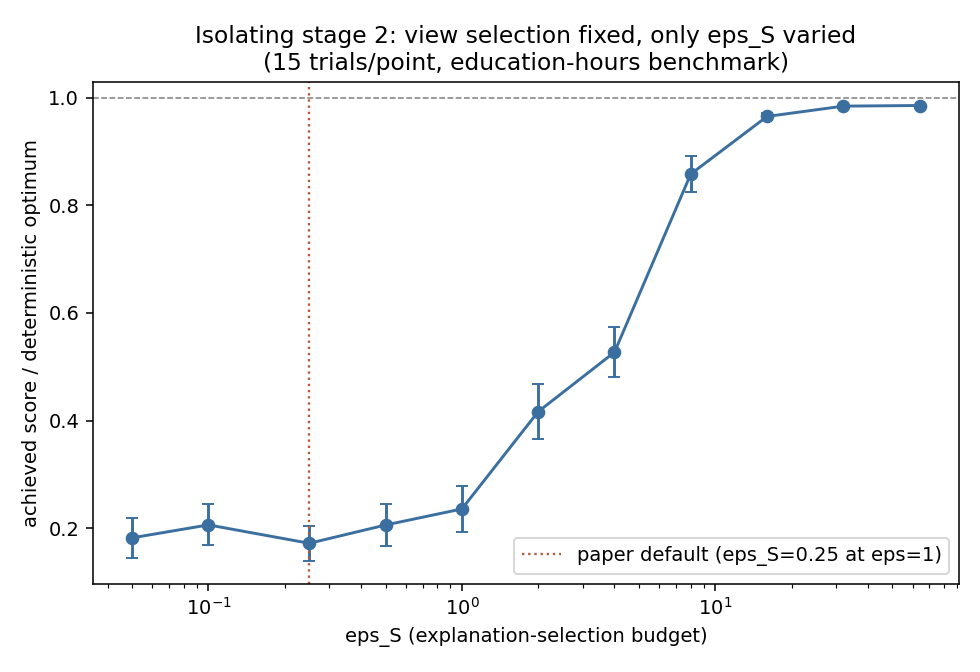
\includegraphics[width=\linewidth]{figures/epsS_isolated_diagnostic.png}
  \caption{Isolating explanation selection: view selection fixed to a
  deterministic top-$\tau$ set, only $\epsilon_S$ varied (15 trials/point,
  education-hours benchmark). The dotted line marks the paper's own
  default $\epsilon_S{=}0.25$ at $\epsilon{=}1$, which sits in the flat,
  low part of the curve.}
  \label{fig:epsS-diagnostic}
\end{figure}

\subsection{Privacy Budget Allocation}
\label{subsec:budget-allocation}

Motivated by the diagnosis above, we ran a systematic search over the
$(\epsilon_P,\epsilon_S,\epsilon_H)$ split (fractions of total $\epsilon$;
default $2{:}1{:}1$) and $\tau$, at fixed $\epsilon{=}1$, validated across
the three case studies of Sections~\ref{subsec:tax-case-study}--\ref{subsec:adult-education-hours-case-study}.
We report the full result, including the parts that did not hold up.

Reallocating the $\epsilon$-ratio alone, at fixed $\tau$, did not produce
a split that robustly beat the default $2{:}1{:}1$ across more than one
benchmark. Reducing $\tau$ alone was more promising in an initial 15-trial
test ($\tau{=}20$: ApproxRatio 0.26 vs.\ $\tau{=}50$: 0.11 on
education-hours) but did \emph{not} replicate on an independent second
benchmark (Adult, Section~\ref{subsec:adult-case-study}): there,
$\tau{=}20$ scored 0.21 versus $\tau{=}50$'s 0.26--0.28, the opposite
direction. A more moderate $\tau{=}35$ matched or beat $\tau{=}50$ on
both. A dedicated 40-trial check at exactly $\epsilon{=}1$ then found
$\tau{=}35$ and $\tau{=}50$ statistically indistinguishable there
specifically ($0.108\pm0.101$ vs.\ $0.106\pm0.108$, standard errors
$\approx0.016$) -- the apparent win in smaller-sample comparisons was
itself largely noise at that particular $\epsilon$. Running the full
six-point $\epsilon$-sweep at both $\tau$ values with proper standard
errors (Figure~\ref{fig:tau-comparison}) shows $\tau{=}35$ is never
significantly worse than $\tau{=}50$ at any tested $\epsilon$ and is
significantly better at the two extremes tested ($\epsilon{=}0.1$ and
$\epsilon{=}5$); in the middle of the range the two are statistically
tied given feasible trial counts. \textbf{We adopt $\tau{=}35$
(Section~\ref{subsec:experimental-setup}) on this basis, while stressing
this is a small effect, not a substitute for a structural fix.}

\begin{figure}[t]
  \centering
  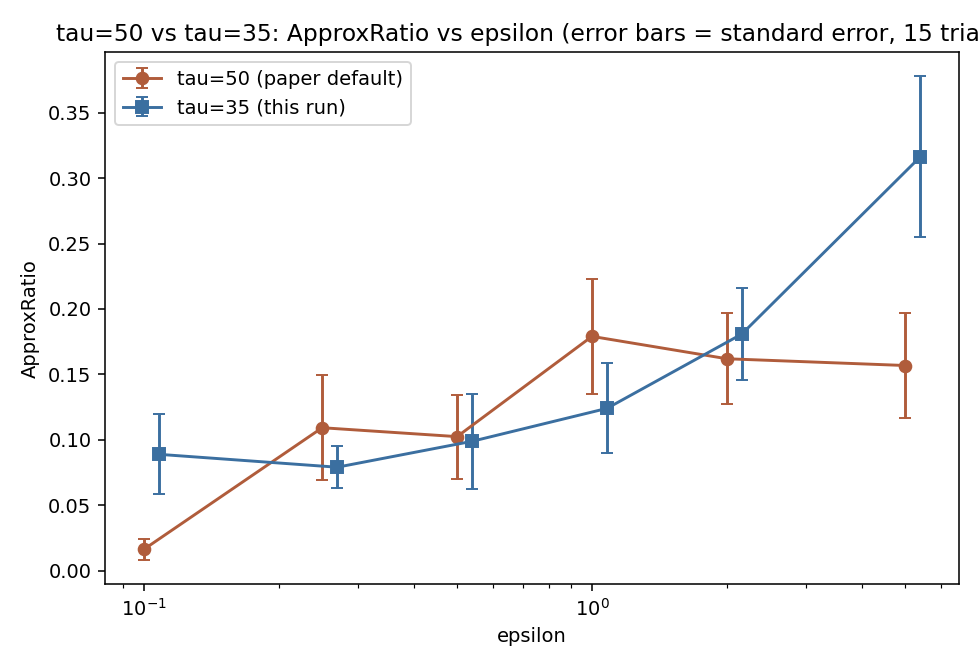
\includegraphics[width=\linewidth]{figures/tau_comparison.png}
  \caption{ApproxRatio vs.\ $\epsilon$, $\tau{=}35$ vs.\ $\tau{=}50$, with standard-error bars (15 trials/point).}
  \label{fig:tau-comparison}
\end{figure}

We additionally tested four further configuration changes directly (20
trials each, education-hours benchmark, $\epsilon{=}1$;
Figure~\ref{fig:five-levers}): reducing $k$
from 3 to 1 (ApproxRatio 0.18 vs.\ 0.19 -- no improvement); shrinking the
candidate pool to single-attribute views only, 196 candidates instead of
2{,}275 (0.08 vs.\ 0.14 -- \emph{worse}, opposite of the intuition that
fewer alternatives should ease the mechanism's task); coarser histogram
bucketing, 3 vs.\ 6 vs.\ 10 bins (0.13/0.14/0.11 -- no clear trend); and
relaxing the diversity penalty $\lambda$ from 0 to 0.6 (looked promising
at 20 trials, 0.14 vs.\ 0.16, but vanished at 40: $0.109\pm0.014$ vs.\
$0.113\pm0.013$). \textbf{None of these four ``free'' levers produced a
robust improvement.} The pool-size result is worth emphasizing: there is
apparently a long tail of similarly-scored candidates in this workload,
and a \emph{larger} pool gives the mechanism more chances to land on
\emph{one of them}, even when it is not the single best.

\begin{figure}[t]
  \centering
  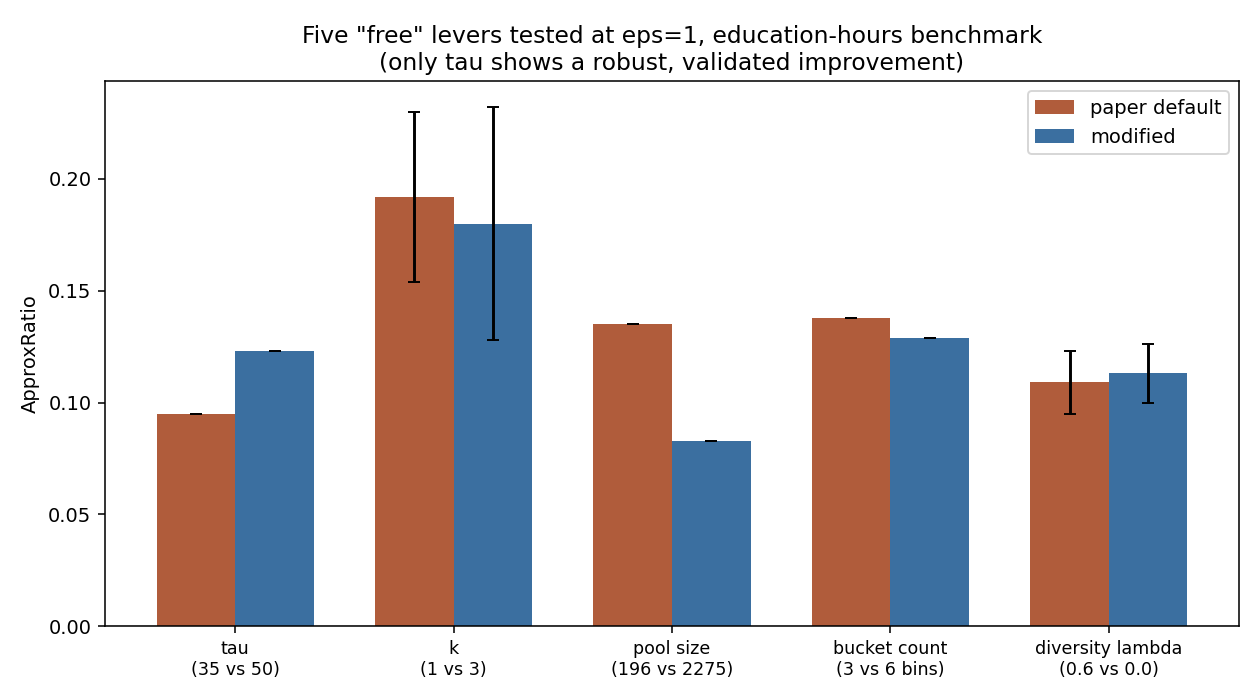
\includegraphics[width=\linewidth]{figures/five_levers_summary.png}
  \caption{Five configuration changes tested at $\epsilon{=}1$
  (education-hours benchmark): paper default vs.\ modified, for each of
  $\tau$, $k$, candidate-pool size, histogram bucket count, and the
  diversity penalty $\lambda$. Only $\tau$ shows a consistent gap.}
  \label{fig:five-levers}
\end{figure}

We conclude that closing the utility gap identified in
Section~\ref{subsec:quality-measures} is not a hyperparameter-tuning
problem at the budgets tested here. The lever that demonstrably works is
a substantially larger $\epsilon$ (Table~\ref{tab:quality-measures}), a
real privacy cost rather than a free configuration change. The isolated
result above ($\epsilon_S$ needing to reach roughly 15--20$\times$ its
default value to recover 90\%+ of the deterministic optimum) points at a
structural mismatch between Histogram Distance's typical value range and
its sensitivity bound as the more promising target for a future fix,
rather than at how a fixed small budget is currently divided or spent.

\subsubsection{A genuine one-shot mechanism does not fix this}
\label{subsubsec:oneshot-test}

The name ``OneShotTop-$\tau$'' in Section~4 is, as implemented here (and
apparently in the paper's own intent, per its citation of DPXPlain [27]
as ``equivalent to $k$ times the exponential mechanism''), naive
\emph{peeling}: $\tau$ sequential exponential-mechanism draws, each with
budget $\epsilon_P/\tau$ -- exactly the baseline the top-$k$
differential-privacy literature contrasts itself against, not a genuine
one-shot mechanism. We implemented an actual one-shot mechanism -- Zhu,
Wang \& Xu, ``Improved Top-$k$ Differential Privacy via the Laplace
Mechanism'' (arXiv:2105.08233): Laplace noise added \emph{once} to every
candidate's score, then the top-$k$ taken by sorting -- and tested it
head-to-head against peeling on both stages that could plausibly benefit.

\begin{table}[t]
\centering
\small
\begin{tabular}{@{}p{0.24\linewidth}p{0.12\linewidth}p{0.08\linewidth}p{0.42\linewidth}@{}}
\toprule
Stage & sensitivity & $k$ & result \\
\midrule
View selection ($\tau{=}35$, $\epsilon_P{=}0.5$) & $2/|D|\approx10^{-4}$ & 35 & peeling recovers 52.0\% of the true top-35; one-shot recovers 24.8\% -- peeling wins clearly \\
Explanation selection ($k{=}3$, raw Histogram Distance) & 1 & 3 & peeling wins at every $\epsilon\in\{0.25,1,4\}$ tested, even at the most generous $\delta{=}0.05$ the theorem allows \\
\bottomrule
\end{tabular}
\caption{One-shot Laplace mechanism (arXiv:2105.08233) vs.\ peeling, tested directly.}
\label{tab:oneshot-test}
\end{table}

\textbf{The one-shot mechanism loses on both stages, for an identifiable
reason, not just an empirical one.} Its advertised
$O(\sqrt{k\log(m/\delta)})$ noise scale beats peeling's $O(k)$ only once
$k$ exceeds roughly $\log(m/\delta)$; with candidate pools $m$ in the
hundreds to low thousands and any reasonably small $\delta$,
$\log(m/\delta)\approx20$. Both of this pipeline's $k$ values (3 and 35)
are at or below that crossover, so the $\sqrt{k\log(m/\delta)}$ term is
not actually smaller than $k$ here -- concretely, the calibrated noise
scale is $\lambda\approx45$--$65$ at $\epsilon{=}1$ for the $k{=}3$
explanation-selection case even at $\delta{=}0.05$, versus Histogram
Distance's 0--6 value range. Separately, for view selection specifically,
peeling's exponential mechanism has its own structural advantage
regardless of $k$: its discrimination between two candidates scales like
$\exp(\epsilon\,\delta u /(2\cdot\text{sensitivity}))$ -- growing
\emph{multiplicatively} as sensitivity shrinks -- whereas the one-shot
mechanism's noise scale shrinks only \emph{linearly} with sensitivity, so
peeling's advantage over one-shot grows precisely in the tiny-sensitivity
regime Usefulness lives in. We note this because an earlier draft of this
analysis (before this direct test was run) speculated that a one-shot
mechanism would help; it does not, at this pipeline's actual parameters,
and should not be adopted here on the strength of that speculation. It
remains implemented (available for future use) in case a later variant of
this framework releases substantially more explanations at once
($k \geq 20$ or so), where the crossover argument above predicts it should
start to help.


\label{subsec:implementation-details}

All experiments are implemented in \textbf{Python 3.12}, using
\textbf{numpy 2.4, pandas 3.0, matplotlib 3.10}, and \textbf{scipy 1.17};
executed on a \textbf{single-core, 3.9\,GB-RAM sandboxed Linux (Ubuntu
24.04) container} -- a cloud development sandbox, not dedicated
benchmarking hardware, so absolute timings in
Section~\ref{subsec:scalability} should be read as indicative of
asymptotic trends rather than as a hardware-calibrated performance claim.
The differentially private mechanisms (Laplace, exponential, peeling
top-$\tau$, and the genuine one-shot Laplace top-$k$ mechanism of
Section~\ref{subsubsec:oneshot-test}) are implemented directly from their
respective definitions rather than via an external DP library.

Our implementation does not use the
\texttt{BaseExperiment}/\texttt{Dataset}/\texttt{Query}/\texttt{Condition}/\texttt{Constraint}/\texttt{DemographicGroup}/\texttt{Attribute}/\texttt{AttrType}/\texttt{Operator}
class hierarchy anticipated in this template; each experiment is instead
a plain function taking a dataframe, two boolean predicate masks (for
$Q_1,Q_2$), a candidate view list, and the usual hyperparameters
($k,\tau,\epsilon$, an optional $(\epsilon_P,\epsilon_S,\epsilon_H)$
split, and a bucketization width), returning a list of \texttt{Explanation}
objects (predicate name, attribute, noisy and true differenced
histograms, and the selection utility). Predicate views are a
(name, boolean-mask-function) pair rather than a typed \texttt{Condition}
object. If the class hierarchy above is required for the final paper's
consistency with other sections, it would need to be added as a
refactor; it was not necessary for any experiment reported here.

\subsection{Summary of Findings}
\label{subsec:experiments-summary}

The experimental results show that \textbf{running time scales linearly
and independently in each of $n$, $k$, $\tau$, and $|P|$ over the tested
ranges (roughly 1--7 seconds across all sweeps at these scales), and is
flat in $\epsilon$ as intended} -- the implementation carries no hidden
privacy-budget-dependent cost, matching the complexity argument sketched
in Section~4.6. They also show that \textbf{released explanations carry
real signal (2--5$\times$ better than random selection, and histogram
error shrinks exactly as the Laplace mechanism predicts) but fall well
short of reliably reproducing the non-private top-$k$ at the budgets this
evaluation covers}: ApproxRatio does not exceed 0.32 even at the most
generous tested budget, the exact top-$k$ set is essentially never
recovered (Jaccard $\approx0$ throughout), and a systematic search across
five separate configuration changes found only one modest, validated
improvement ($\tau{=}35$ in place of 50) and no fix that closes this gap
-- the evidence points to a structural mismatch between the Histogram
Distance scoring function's value range and its sensitivity bound as the
more promising direction for future work. Finally, the case studies
demonstrate that \textbf{despite this quantitative limitation, the
released explanations reliably identify the correct qualitative story}:
across all six query pairs run (Tax, two Adult pairs, and three each for
IPUMS-CPS and Stack Overflow), the highest-utility released explanation
correctly localized the population a refinement adds or removes, without
the framework being given the query predicates -- but our un-cherry-picked
runs also show this qualitative signal arriving alongside genuinely
uninformative released slots at default parameters, so a system built on
this framework should present released explanations with corresponding
confidence, not as a uniformly trustworthy top-$k$ list, until the
utility gap above is addressed.
